\chapter{Methodology}

The primary focus of this research is the infodemiological surveillance of three (3) of the top communicable diseases - Measles, Influenza, Typhoid Fever -  in the Philippines, as reported by the Philippines' Department of Health (DOH) \cite{dohrecord2015}. The research is divided into two parts, which are 1) collection of health-related tweets and their visualization in a map, and 2) the modeling and prediction of possible areas of outbreaks based on Twitter posts.

This section breaks down the phases further into five (5) subsections, \textit{Health Data Collection}, \textit{Infodemiological Modeling and Classification}, \textit{Twitter Data Visualization}, \textit{Epidemiological Correlation and Modeling}, and \textit{STEM Scenario Visualization}. The overview of the methodology can be seen in Figure \ref{fig:GeneralMethodology}.


\begin{figure}[!ht]
    \centering
    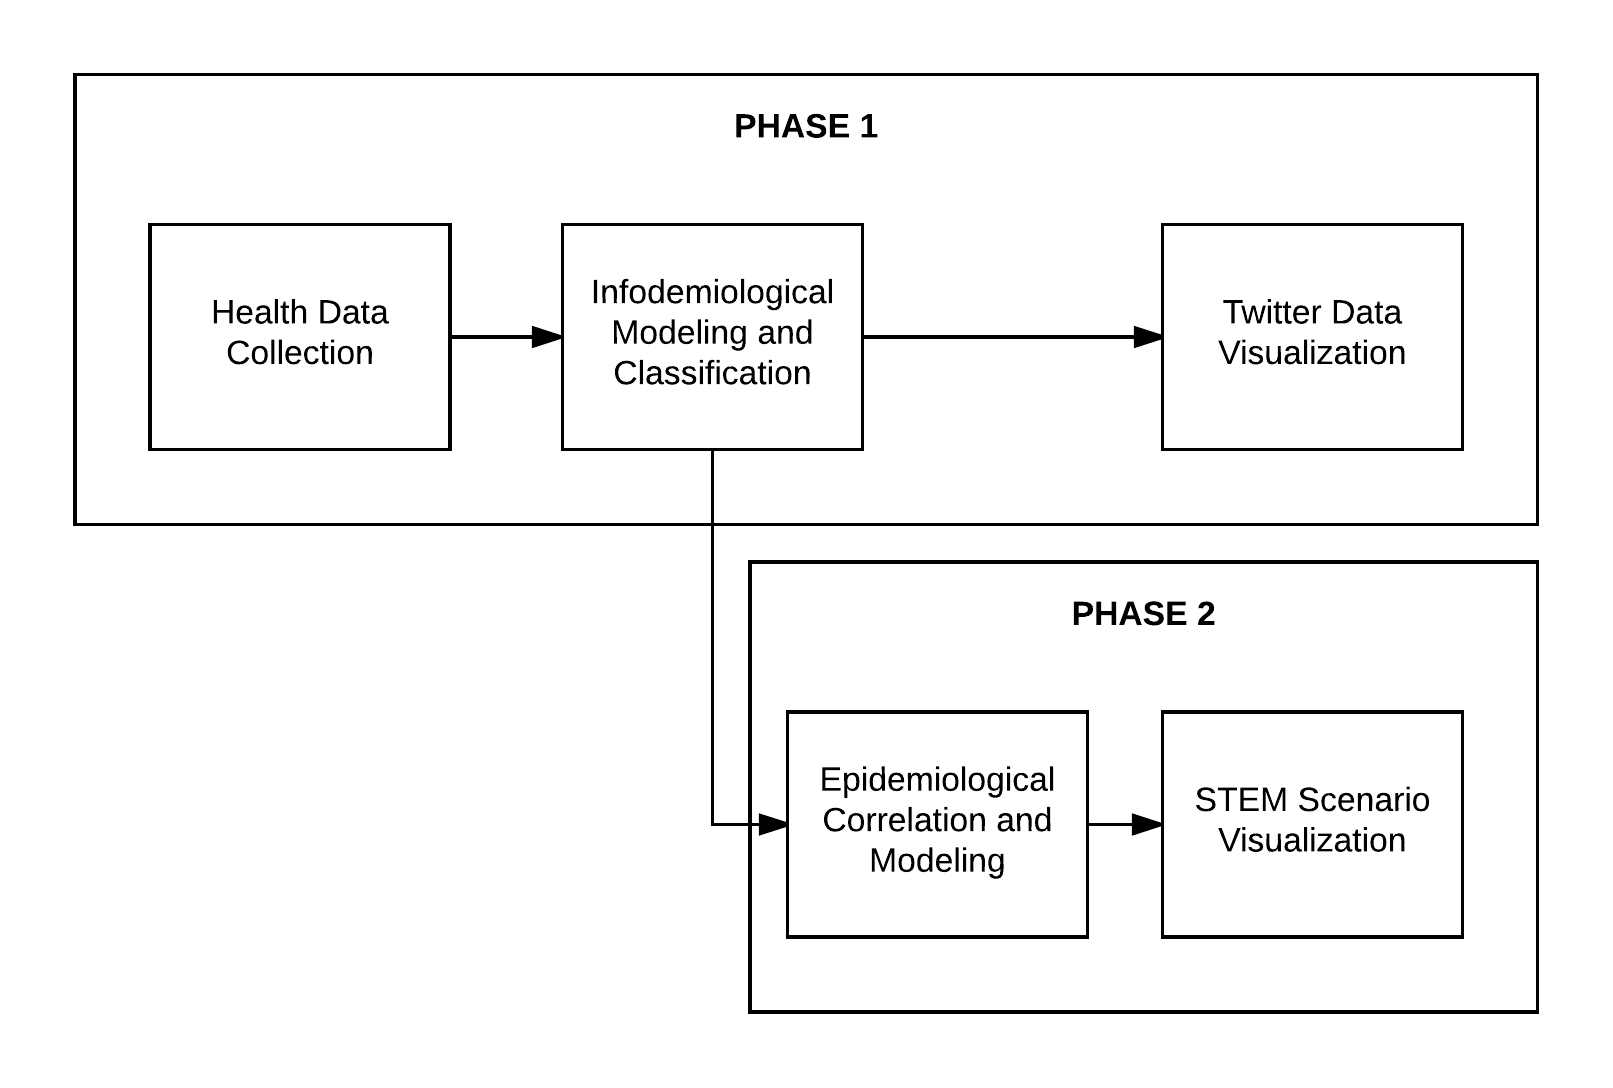
\includegraphics[width=\textwidth]{GeneralMethodology}
	\caption{General view of the research's methodology.}
	\label{fig:GeneralMethodology}
\end{figure}

\section{Health Data Collection}
The data that will be used for the research comes from two (2) sources, which are 1) publicly available individual posts collected from \textbf{Twitter}, which then will be validated through 2) publicly available statistical documents that largely leverages on the data by \textbf{Philippines' Department of Health (DOH)}. The users' posts from Twitter represents majority of the data to be processed, while the supporting records and documents act as a sustained supplementary data to be used as a baseline for comparison, correlation, and prediction.

\subsection{Twitter Data Collection}
Through the use of Twitter's public streaming Advanced Programming Interfaces (API), a tool will be used to gather relevant tweets through using keywords. The tool developed by the Ateneo Java Wireless Competency Center (AJWCC) is the chosen tweet collector that will be used. The tool is based on the \textit{Ruby on Rails} programming language and framework, using the \textit{tweetstream} gem. The tool collects tweets in realtime based on the supplied keywords in its configuration file. It will be deployed on a local server with a constant connection to the Internet. This means that the collection will happen the whole day. The official start of collection for real-time tweet collection will be on \textit{June 13, 2016} until \textit{September 13, 2016}. Added to real-time collection, the research will also be accessing historical tweets through the AJWCC as well.

\subsubsection {Keyword Compilation}
Based on the related literature review, words associated to the disease will be gathered. Listed are possible keyword groups that may be found in social media posts.

\begin{itemize} 
\item \textbf{Coloquial Terms} - Terms used by the people that may indicate the presence of flu.
	\begin{itemize} 
		\item Example: \textit{``lagnat"}, \textit{``flu"}, \textit{``sick"}
	\end{itemize}
\item \textbf{Symptoms} - The symptoms of influenza. This includes both English and Filipino words.
	\begin{itemize} 
		\item Example: \textit{``ubo''}, \textit{``cough''}, \textit{``sipon''}, \textit{``sneeze''}
	\end{itemize}
\item \textbf{Behavior/Actions} - The behavior of people when they have the flu. For example, people  buy medicines during flu seasons, therefore drugstores, in general, may be used as a keyword.
	\begin{itemize} 
		\item Example: \textit{``mercury drug''}, \textit{``stay in bed''}, \textit{``tulog''}, \textit{``gamot''}
	\end{itemize}
\item \textbf{Weather Condition} - Lastly, the weather conditions of an area. Flu seasons arise when it's cold.
\begin{itemize} 
		\item Example: \textit{``rain''}, \textit{``ulan''}, \textit{``cold''}
	\end{itemize}
\end{itemize}

These keywords, along with their conjugations if possible, will be used as the search parameters for Twitter. 

\subsection{Department of Health - Epidemiology Bureau Data}

Regularly, the Philippines' Department of Health publishes through their websites their gathered disease surveillance statistics. This can be accessed by visiting \textit{http://nec.doh.gov.ph/}. Since these data directly come from the DOH, these can be considered as a the gold standard for correlation and regression.

% Besides the published statistics found in the Department of Health's website, through the project headed by Dr. Regina Estuar in cooperation with the DOH's Surveillance in Post Extreme Emergencies and Disasters (SPEED) project \cite{whatisspeed}, data sets can be gathered directly from the department itself to be used in the correlation computation. SPEED is a warning surveillance system used by the DOH after disasters to help in identifying trends in people's health conditions, and ultimately, to help in preventing diseases from spreading \cite{whatisspeed}. Because of the surveillance nature of this project, the data being collected can be considered as an accurate source for correlation with the gathered tweets.
